\documentclass[12pt, a4paper]{article}

\usepackage[utf8]{inputenc}
\usepackage[T1]{fontenc}
\usepackage{polski}

\usepackage[top=2.5cm, bottom=2.5cm, left=2.5cm, right=2.5cm]{geometry}

\usepackage{graphicx}
\usepackage[colorlinks=true, linkcolor=black, urlcolor=blue]{hyperref}
\usepackage{listings}
\usepackage{times}
\usepackage{float}

\lstset{
  language=Java,
  basicstyle=\small\ttfamily,
  keywordstyle=\bfseries\color{blue},
  stringstyle=\color{red},
  commentstyle=\itshape\color{green!40!black},
  breaklines=true,
  showstringspaces=false,
  frame=single,
  numbers=left,
  numberstyle=\tiny\color{gray},
  captionpos=b
}

\begin{document}

\begin{titlepage}
    \begin{flushleft}
        \Large\textbf{UNIWERSYTET RZESZOWSKI} \\
        \normalsize WYDZIAŁ NAUK ŚCISŁYCH I TECHNICZNYCH \\
        \normalsize INSTYTUT INFORMATYKI
    \end{flushleft}
    \hfill
    \begin{flushright}
        
\includegraphics[width=3cm]{UR;-sygnet-niebieski.jpg} 
    \end{flushright}

    \vspace{4cm}

    \begin{center}
        \Large Tomasz Wiśniewski \\
        \normalsize 134986 \\ 
        \normalsize Informatyka
    \end{center}

    \vspace{2cm}

    \begin{center}
        \huge\textbf{System zarządzania turniejami e-sportowymi} \\
        \vspace{1cm}
        \Large Praca projektowa
    \end{center}

    \vfill

    \begin{flushright}
        \normalsize Praca wykonana pod kierunkiem \\
        \normalsize dr Ewa Żesławska
    \end{flushright}

    \vspace{2cm}
    
    \begin{center}
        \normalsize Rzeszów 2025
    \end{center}
\end{titlepage}

\newpage
\tableofcontents
\newpage

\listoffigures
\listoftables
\listoflistings
\newpage

\section*{Streszczenie}
\addcontentsline{toc}{section}{Streszczenie}
Niniejszy projekt opisuje proces tworzenia oraz implementacji aplikacji desktopowej "System zarządzania turniejami e-sportowymi". Aplikacja została napisana w języku Java z wykorzystaniem biblioteki Swing do budowy graficznego interfejsu użytkownika. Głównym celem systemu jest automatyzacja i uproszczenie procesu zarządzania rozgrywkami turniejowymi. Projekt wykorzystuje architekturę warstwową, w tym wzorzec DAO do komunikacji z relacyjną bazą danych SQLite za pośrednictwem JDBC, a kluczowym elementem implementacji jest zastosowanie hierarchii dziedziczenia do modelowania różnych typów drużyn.

\vspace{1cm}
\section*{Abstract}
\addcontentsline{toc}{section}{Abstract}
This project describes the development and implementation process of a desktop application, "Esports Tournament Management System". The application was written in the Java language using the Swing library for the graphical user interface. The main objective of the system is to automate and simplify the management of tournament gameplay. The project utilizes a layered architecture, including the DAO pattern for communication with a relational SQLite database via JDBC. A key element of the implementation is the use of an inheritance hierarchy to model different types of teams participating in the tournament.

\newpage

\section{Opis założeń projektu}
Celem projektu było stworzenie w pełni funkcjonalnego systemu informatycznego do zarządzania turniejami e-sportowymi. Głównym problemem, który aplikacja ma rozwiązywać, jest brak prostych i dostępnych narzędzi dla organizatorów amatorskich lub lokalnych rozgrywek. Obecnie osoby te często polegają na skomplikowanych arkuszach kalkulacyjnych lub ręcznych zapiskach, co jest nieefektywne i podatne na błędy. Problem ten jest ważny, ponieważ scena amatorskiego e-sportu dynamicznie się rozwija, a bariery organizacyjne ograniczają jej potencjał.

Aby rozwiązać ten problem, niezbędne było stworzenie aplikacji, która automatyzuje kluczowe procesy. Realizacja projektu przebiegała krok po kroku: od zaprojektowania architektury i bazy danych, przez implementację logiki zarządzającej turniejem, aż po stworzenie intuicyjnego interfejsu graficznego. Wynikiem prac jest samodzielna aplikacja desktopowa, która minimalizuje nakład pracy organizatora i zapewnia integralność oraz poprawność przebiegu rozgrywek.

Aplikacja została zaprojektowana z myślą o turniejach w popularnej grze e-sportowej Valorant. W standardowym meczu rywalizują dwie pięcioosobowe drużyny, a celem jest wygranie 13 rund. Pojedynczą rundę można wygrać poprzez wyeliminowanie wszystkich przeciwników lub przez podłożenie i zdetonowanie bomby (zwanej "Spike") przez stronę atakującą. Mecz kończy się, gdy jedna z drużyn jako pierwsza osiągnie 13 punktów, co prowadzi do wyników takich jak 13-10 czy 13-5. Zrozumienie tej prostej zasady punktacji jest kluczowe dla kontekstu działania aplikacji, która pozwala na zapisywanie i przetwarzanie właśnie takich wyników.

\subsection{Wymagania funkcjonalne}
\begin{itemize}
    \item \textbf{Zarządzanie danymi turnieju:} System pozwala na dodawanie i usuwanie drużyn różnych typów (Profesjonalna, Amatorska, etc.) oraz przypisanych do nich graczy.
    \item \textbf{Automatyzacja rozgrywki:} System automatycznie generuje pary meczowe w poszczególnych etapach turnieju, uwzględniając losowość i obsługując przypadki nieparzystej liczby drużyn poprzez mechanizm "wolnego losu".
    \item \textbf{Zarządzanie wynikami:} Interfejs umożliwia wprowadzanie wyników zakończonych meczów.
    \item \textbf{Przebieg turnieju:} Aplikacja automatycznie zarządza przechodzeniem do kolejnych etapów po zakończeniu rundy, włączając w to logikę meczu o 3. miejsce.
    \item \textbf{Funkcje administracyjne:} System posiada funkcję całkowitego resetu turnieju, która usuwa wszystkie dane z bazy.
    \item \textbf{Generowanie raportów:} Aplikacja umożliwia wgląd w historię wszystkich rozegranych meczów oraz prezentuje finalny ranking po zakończeniu turnieju.
\end{itemize}

\subsection{Wymagania niefunkcjonalne}
\begin{itemize}
    \item \textbf{Wydajność:} Operacje interfejsu oraz podstawowe zapytania do bazy danych powinny być wykonywane w czasie poniżej 2 sekund, zapewniając płynność działania.
    \item \textbf{Użyteczność:} Interfejs użytkownika został zaprojektowany w sposób prosty i intuicyjny, aby był zrozumiały dla użytkownika bez wiedzy technicznej.
    \item \textbf{Niezawodność:} Aplikacja jest odporna na podstawowe błędy użytkownika (np. próba startu turnieju bez drużyn) i obsługuje je, wyświetlając odpowiednie komunikaty.
    \item \textbf{Przenośność:} Program napisany w Javie jest przenośny i działa na każdym systemie operacyjnym (Windows, macOS, Linux), na którym zainstalowano środowisko JRE.
    \item \textbf{Utrzymywalność:} Kod źródłowy został podzielony na logiczne warstwy (model, DAO, core, ui), co ułatwia jego zrozumienie, konserwację i ewentualny dalszy rozwój.
\end{itemize}

\section{Opis struktury projektu}
Projekt został zrealizowany w języku Java z wykorzystaniem biblioteki Swing do stworzenia graficznego interfejsu użytkownika. Warstwa persystencji danych opiera się na plikowej bazie SQLite, z którą aplikacja komunikuje się poprzez API JDBC.

\subsection{Architektura aplikacji}
Struktura projektu została oparta na architekturze warstwowej w celu separacji poszczególnych logik:
\begin{itemize}
    \item \textbf{Pakiet \texttt{model}} - zawiera klasy danych, w tym abstrakcyjną klasę \texttt{Druzyna} oraz jej cztery konkretne podklasy (\texttt{DruzynaProfesjonalna}, \texttt{DruzynaAmatorska}, etc.), które tworzą wymaganą hierarchię dziedziczenia.
    \item \textbf{Pakiet \texttt{dao}} - (Data Access Object) - Zestaw klas odpowiedzialnych za całą komunikację z bazą danych, hermetyzujących zapytania SQL.
    \item \textbf{Pakiet \texttt{core}} - Rdzeń aplikacji, zawierający główną logikę biznesową w klasie \texttt{TournamentManager}.
    \item \textbf{Pakiet \texttt{ui}} - Warstwa prezentacji, odpowiedzialna za graficzny interfejs użytkownika (\texttt{TournamentGUI}).
\end{itemize}

\subsection{Schemat bazy danych}
System wykorzystuje plikową bazę danych SQLite do przechowywania danych. Składa się ona z trzech głównych tabel:
\begin{enumerate}
  \item \textbf{druzyna}: Przechowuje informacje o drużynach (id, nazwa, typ, sponsor, miasto, itd.).
  \item \textbf{gracz}: Przechowuje informacje o graczach (id, nick, druzyna\_id).
  \item \textbf{mecz}: Przechowuje historię rozegranych meczów (id, id drużyn, wyniki, zwycięzca).
\end{enumerate}

\begin{figure}[H]
 \centering
 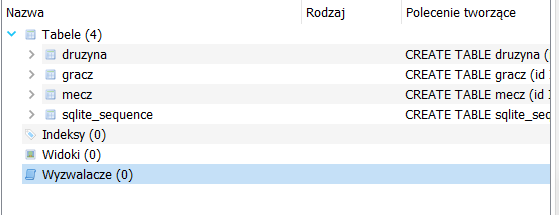
\includegraphics[width=0.8\textwidth]{rysunek5.png}
 \caption{Struktura tabel w bazie danych \texttt{turniej.db}.}
 \label{fig:schemat_bazy}
\end{figure}

\subsection{Wymagania sprzętowe i oprogramowanie}
\begin{itemize}
    \item \textbf{System operacyjny:} Windows, macOS lub Linux.
    \item \textbf{Oprogramowanie:} Zainstalowane środowisko Java Development Kit (JDK) w wersji 11 lub nowszej.
    \item \textbf{Biblioteki zewnętrzne:} Do poprawnego działania aplikacji wymagane jest dołączenie do struktury projektu sterownika JDBC dla SQLite. W projekcie wykorzystano plik \textbf{\texttt{sqlite-jdbc-3.40.1.0.jar}}, który jest dołączony do plików źródłowych.
    \item \textbf{Pamięć RAM:} Minimum 256 MB.
    \item \textbf{Miejsce na dysku:} Około 50 MB.
\end{itemize}

\section{Harmonogram realizacji projektu}
\subsection{Przebieg prac}
Realizacja projektu została podzielona na cztery główne fazy, rozłożone w czasie. Poniższa tabela przedstawia uproszczony harmonogram prac, który stanowi podstawę do stworzenia diagramu Gantta.
\begin{table}[H]
\centering
\begin{tabular}{|l|p{9cm}|}
\hline
\textbf{Faza projektu} & \textbf{Główne zadania} \\ \hline
1. Analiza i Projekt & Analiza wymagań, projekt architektury, schemat bazy danych. \\ \hline
2. Implementacja Rdzenia & Kodowanie modelu, DAO, logiki w \texttt{TournamentManager}. \\ \hline
3. Implementacja GUI & Budowa interfejsu w Swing, połączenie z logiką. \\ \hline
4. Testowanie i Dokumentacja & Testowanie funkcjonalności, poprawa błędów, pisanie dokumentacji. \\ \hline
\end{tabular}
\caption{Uproszczony harmonogram realizacji projektu.}
\label{tab:harmonogram}
\end{table}

\subsection{Problemy napotkane podczas realizacji}
W trakcie implementacji napotkano kilka wyzwań logicznych. Największym z nich była poprawna obsługa przypadków brzegowych w logice turnieju, takich jak start z nieparzystą liczbą drużyn. Początkowa wersja algorytmu błędnie obsługiwała "wolny los", co wymagało gruntownej przebudowy metody zarządzającej przejściem między etapami. Kolejnym problemem była konfiguracja połączenia z bazą danych, co objawiało się błędem "No suitable driver found" i zostało rozwiązane poprzez poprawne dodanie sterownika JDBC do zależności projektu.

\subsection{System kontroli wersji}
Kod źródłowy projektu był zarządzany przy użyciu systemu kontroli wersji Git. Repozytorium publiczne projektu znajduje się pod adresem: \url{https://github.com/Wisniewsky/programowanie-obiektowe}

\section{Prezentacja warstwy użytkowej projektu}
Aplikacja została zaprojektowana z myślą o prostocie obsługi. Główny interfejs podzielony jest na trzy części: panel zarządzania po lewej, drabinkę turnieju na środku i panel akcji po prawej.

\begin{figure}[H]
 \centering
 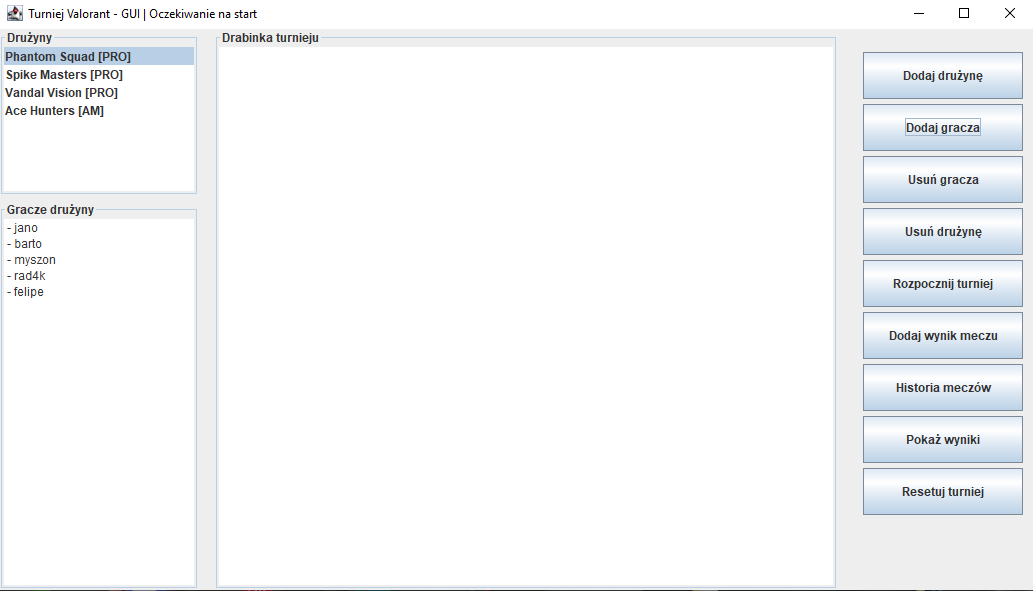
\includegraphics[width=0.9\textwidth]{dzialanie_programu_1.png}
 \caption{Główne okno aplikacji po uruchomieniu.}
 \label{fig:glowne_okno}
\end{figure}

Aby dodać drużynę, należy kliknąć przycisk "Dodaj drużynę" i wypełnić formularz, który pojawi się w nowym oknie. 

\begin{figure}[H]
 \centering
 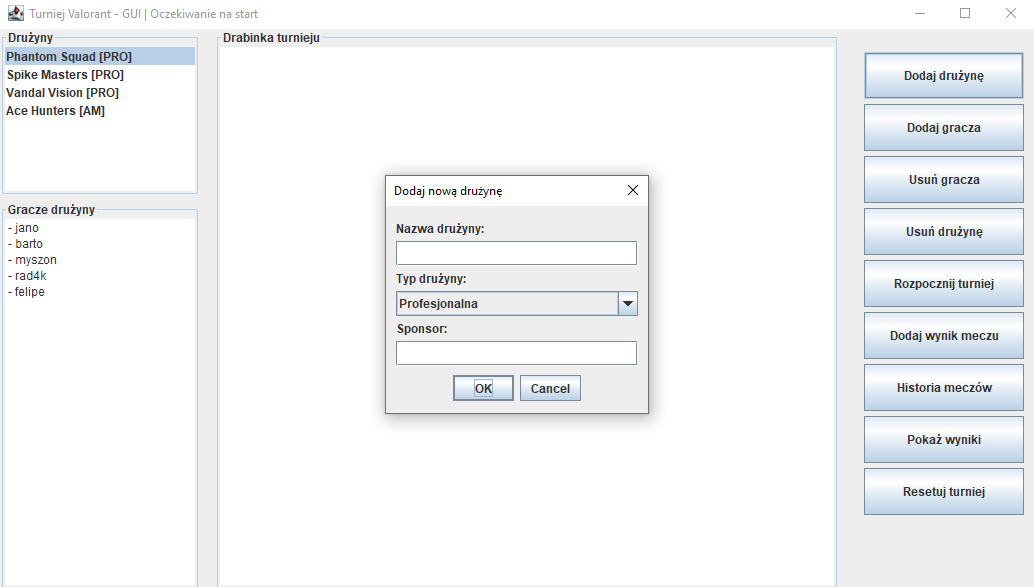
\includegraphics[width=0.7\textwidth]{rysunek2.png}
 \caption{Formularz dodawania nowej drużyny typu "Profesjonalna".}
 \label{fig:dodaj_druzyne}
\end{figure}

Po dodaniu co najmniej trzech drużyn, można rozpocząć turniej przyciskiem "Rozpocznij turniej", co spowoduje wygenerowanie pierwszego etapu, wylosowanie par i puli map.

\begin{figure}[H]
 \centering
 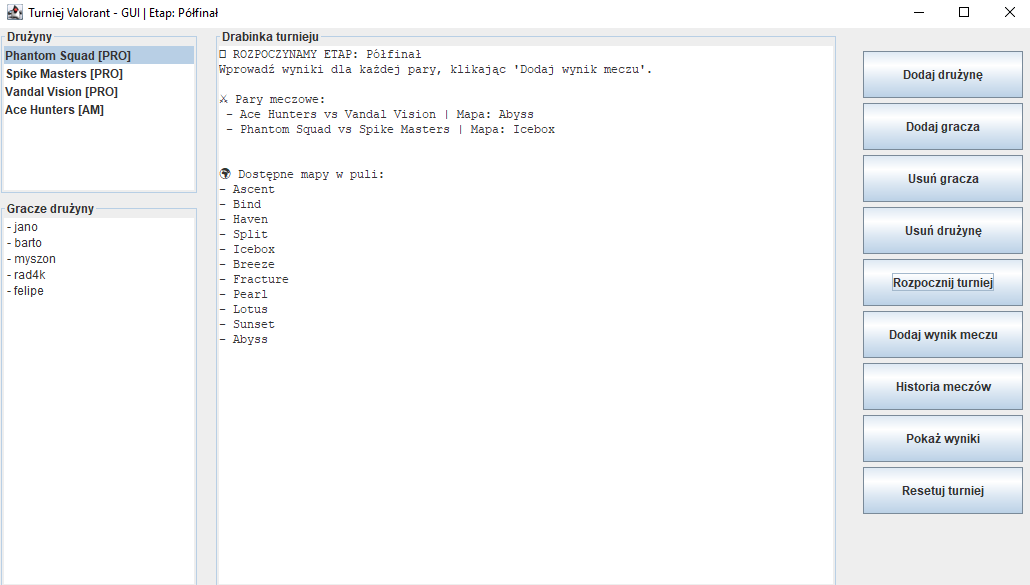
\includegraphics[width=0.9\textwidth]{rysunek3.png} 
 \caption{Widok drabinki turniejowej po wylosowaniu par i puli map.}
 \label{fig:drabinka}
\end{figure}

Wprowadzanie wyników odbywa się za pomocą przycisku "Dodaj wynik meczu". Po zakończeniu rundy i całego turnieju, możliwe jest wyświetlenie okna z podsumowaniem wyników.

\begin{figure}[H]
 \centering
 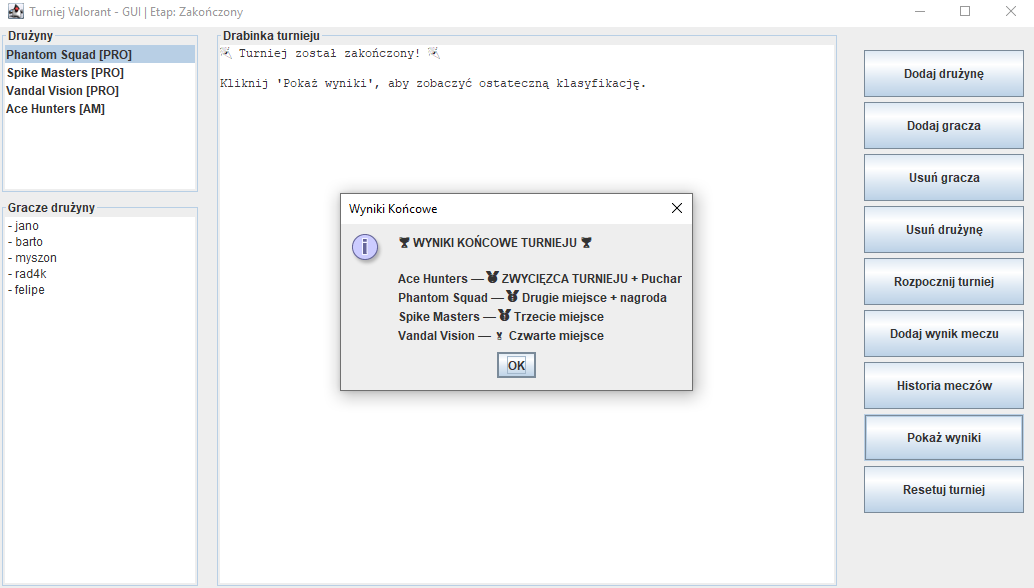
\includegraphics[width=0.6\textwidth]{rysunek4.png} 
 \caption{Okno prezentujące końcowe wyniki turnieju.}
 \label{fig:wyniki}
\end{figure}

\section{Podsumowanie}
Zrealizowany projekt z powodzeniem implementuje system do zarządzania turniejami e-sportowymi. Aplikacja spełnia wszystkie założone wymagania funkcjonalne, oferując stabilne i logicznie działające środowisko do prowadzenia rozgrywek. Najważniejszym osiągnięciem projektowym jest implementacja elastycznej logiki turniejowej oraz zbudowanie obiektowej architektury opartej na hierarchii dziedziczenia.

Aplikacja stanowi solidną bazę do dalszego rozwoju. W przyszłości można by ją rozbudować o takie funkcjonalności jak: pełna implementacja operacji CRUD (w tym edycja danych), import i eksport danych z/do plików CSV, czy też bardziej zaawansowane statystyki graczy i drużyn.

\newpage
\section*{Bibliografia}
\addcontentsline{toc}{section}{Bibliografia}
\begin{enumerate}
    \item Materiały dydaktyczne z kursu "Programowanie Obiektowe Java", dr Ewa Żesławska, Uniwersytet Rzeszowski, 2025.
\end{enumerate}

\appendix
\section{Oświadczenie o samodzielności pracy}

\begin{figure}[H]
 \centering
 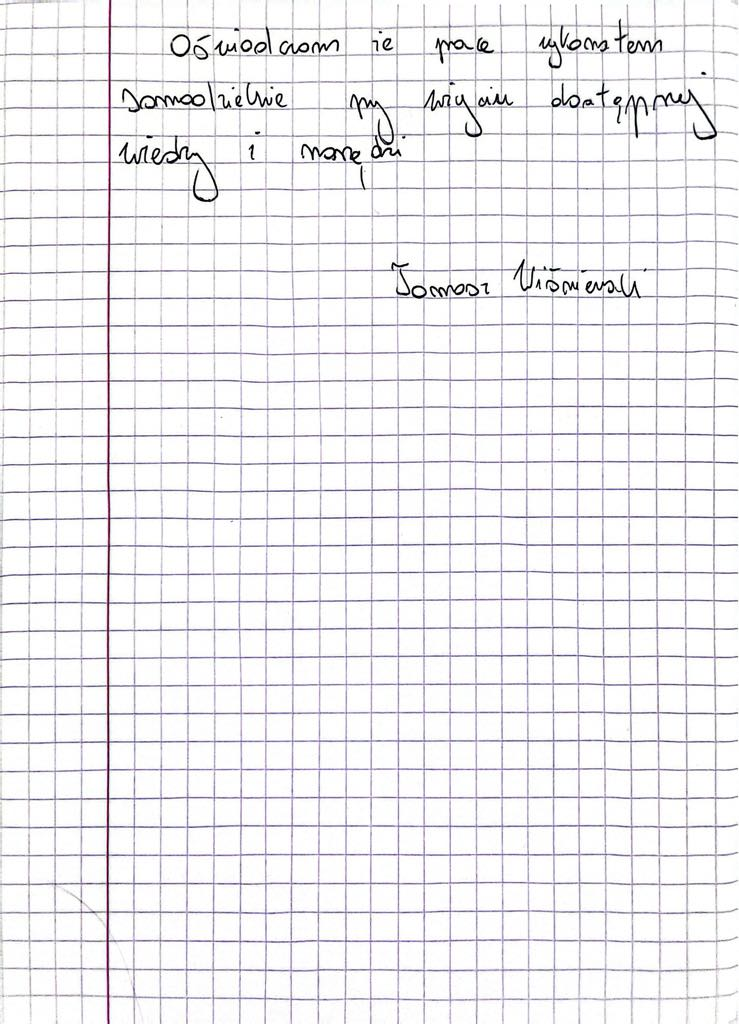
\includegraphics[width=\textwidth]{oswiadczenie.jpeg}
 \caption{Oświadczenie o samodzielności wykonania pracy.}
 \label{fig:oswiadczenie}
\end{figure}

\end{document}